\section{Common Manuscript Mistakes}

Manuscript follows a strict set of rules and conventions, however there are a \emph{lot} of them and as such it's perfectly natural that children struggle to remember them all, resulting in mistakes.

Since there's not a huge amount of point attempting to build a system to recognise something it will never come across,I needed to establish exactly which mistakes were actually likely to occur, for which I referred to two main sources.

The first is Music Theory in Practice, \parencite{taylor2008music} which was mentioned in \cref{sec:music-book-taylor2008}. It's a book specifically written to teach music theory and has some great examples of mistakes a student should avoid.

My second source was real professional musicians and tutors but this involved a more complex method which is covered in \cref{sec:teacher-data-gathering}.

\subsection{Gathering Professional Feedback}
\label{sec:teacher-data-gathering}

In order to build an application which can help to compensate for the absence of a tutor, we need to ensure that it can spot as many of the same mistakes as a tutor would.

The most logical way to establish precisely what these mistakes are is (surprise surprise) to ask the tutors, however when I did this, several of them found it difficult to express the mistakes they had seen children make without a piece of music in front of them.

I therefore devised the following method for gathering mistake data:

\begin{itemize}
  \item Build the input section of the application such that a student can `free-draw' on a blank music staff.
  \item Set the student challenges and ask them to have a go at as many as they can
  \item Print out the attempts (labelled) and get a music tutor to mark them freely
\end{itemize}

To save time (and paper) the marking was done 3-UP on a portrait sheet of A4, an example of one of the tutor feedback sheets can be seen in \cref{fig:teacher-sheet}. It should be noted that in some of the feedback tutors refer to errors differently, for example by using `the stem is on the wrong side' to mean that either a note stem is up when it should be down or that it's on the right when it should be on the left.

\begin{figure}[H]
  \centering
  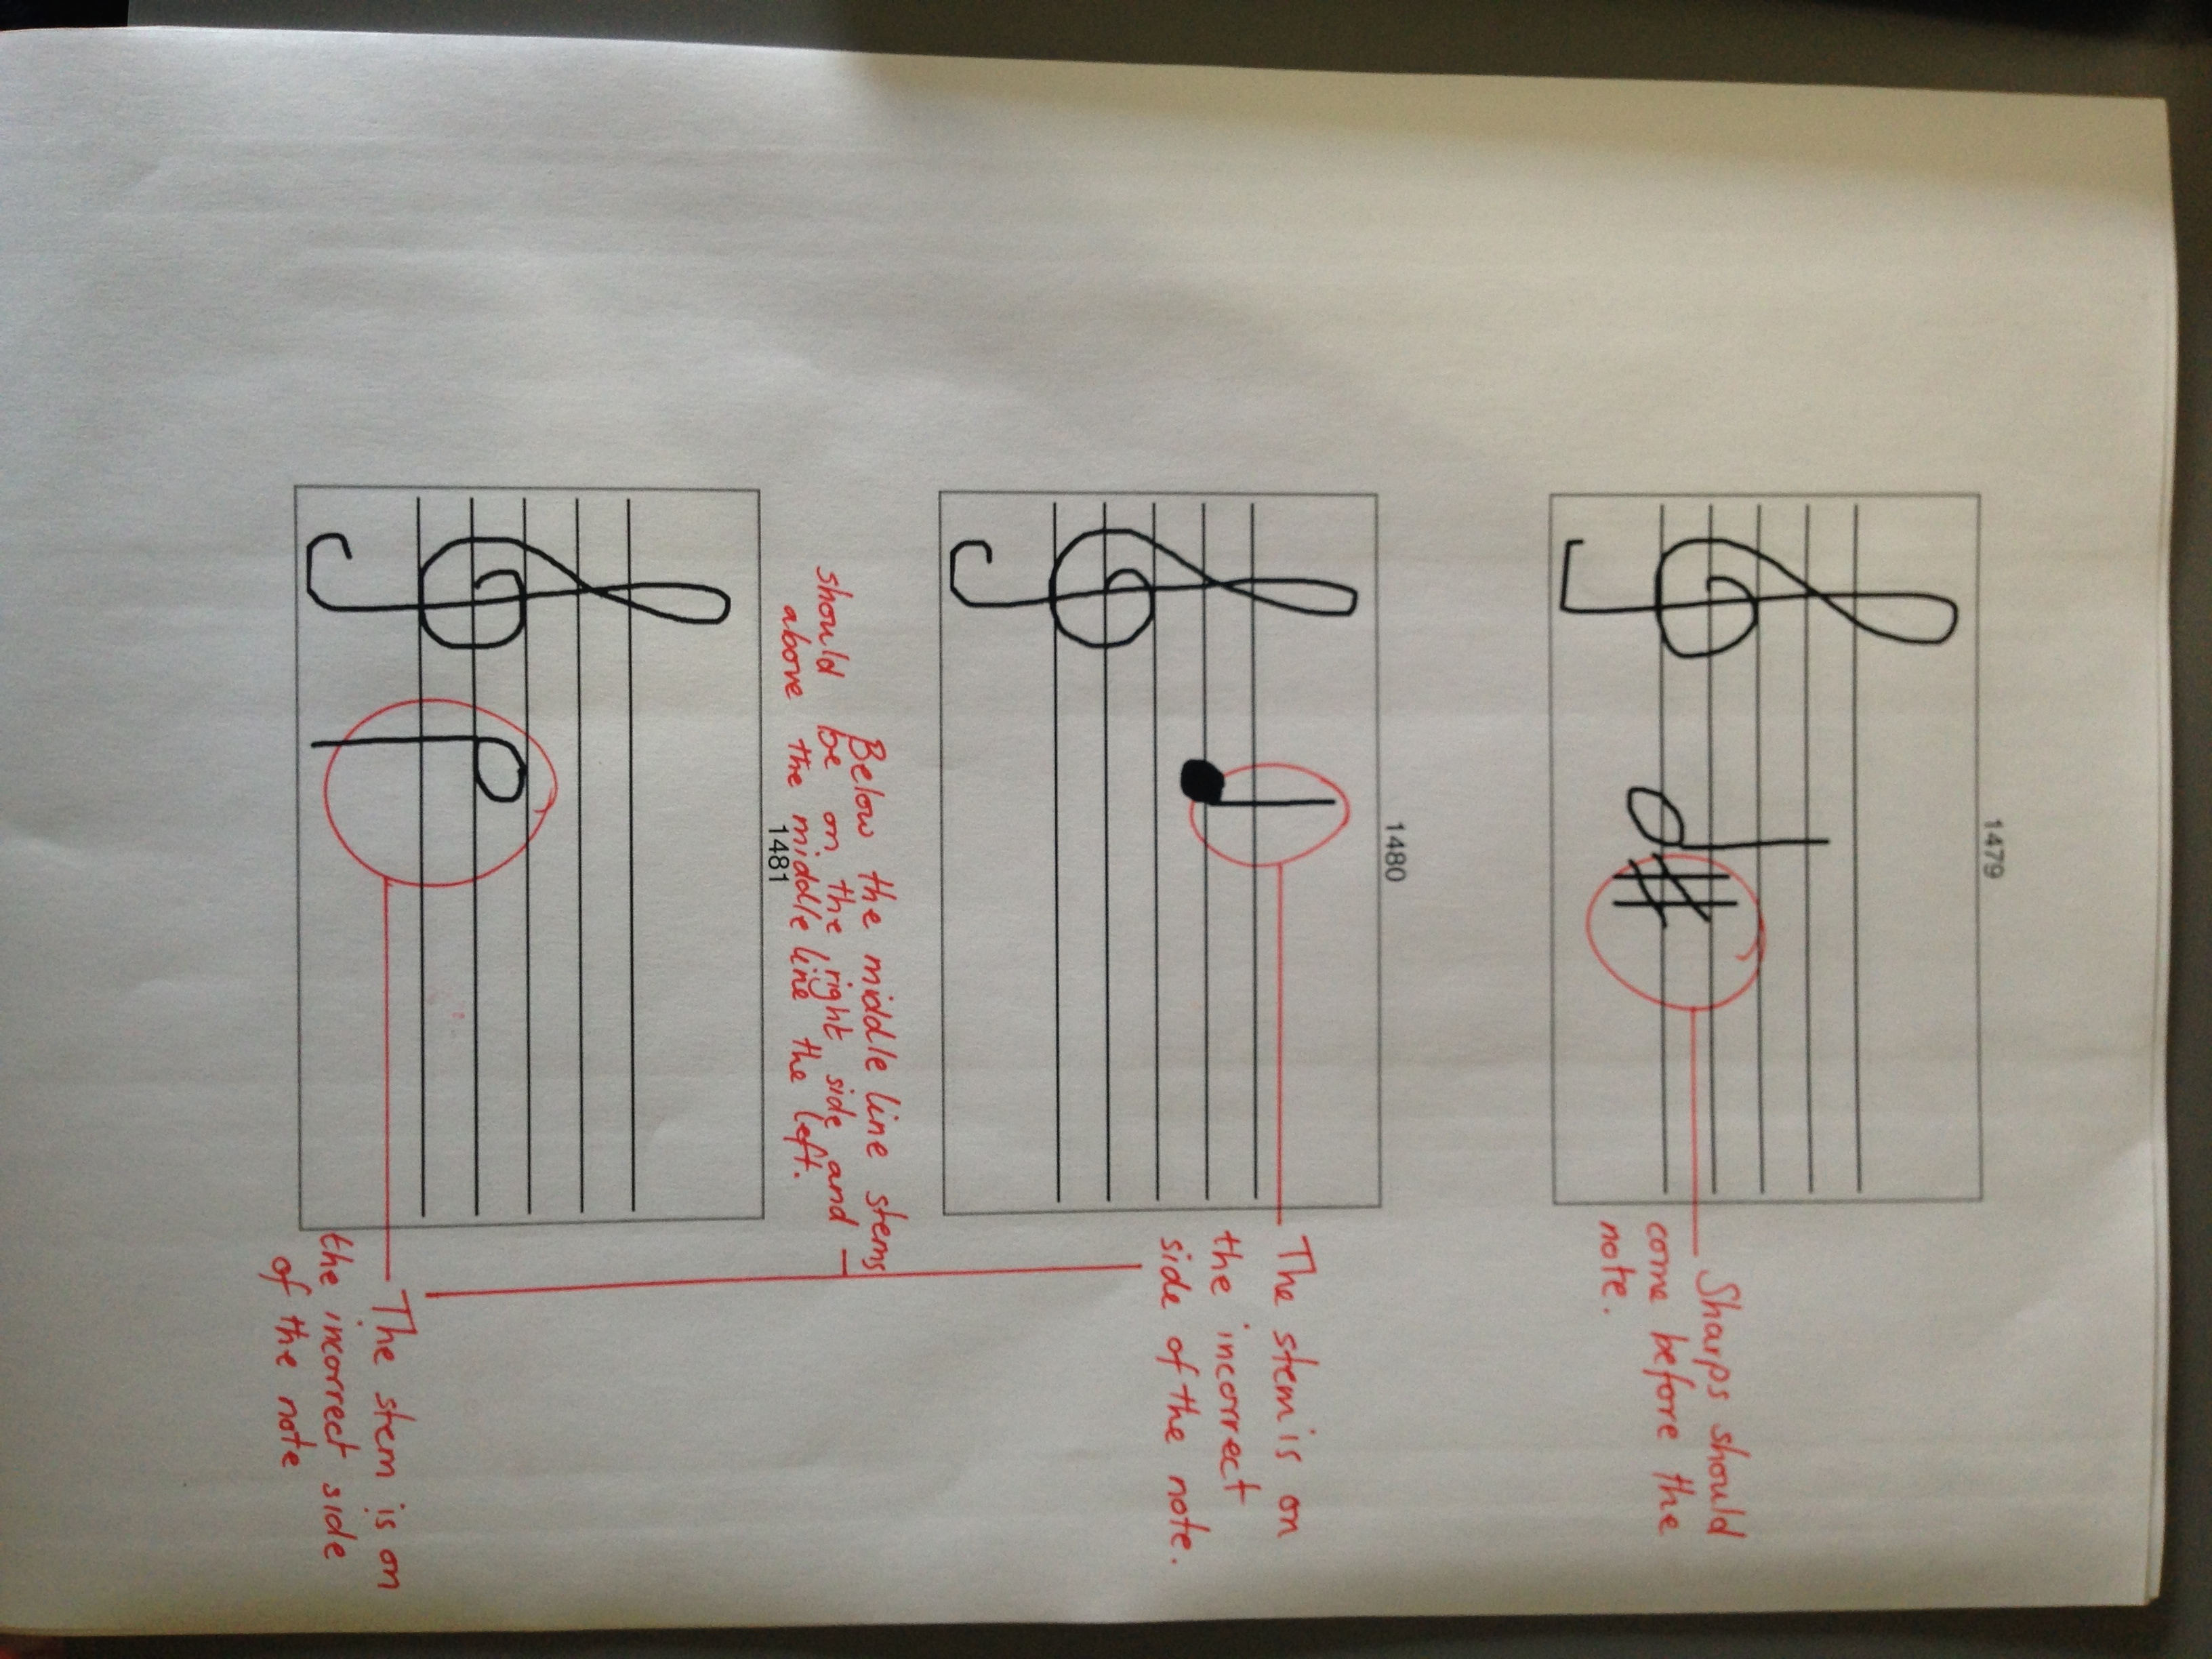
\includegraphics[width=\linewidth]{gfx/photos/teacher-sheet-1.jpg}
  \caption{Example of tutor-annotated manuscript}
  \label{fig:teacher-sheet}
\end{figure}

Once this data was collected I had a sample of \todo{COUNT HOW MANY STUDENT SAMPLES I HAD} marked samples \todo[inline,color=blue]{Put this full dataset at the end?} and I was able to extract some recurring issues. I present some of them below and later on in \cref{sec:scoring} I go over how I spot these mistakes.

\subsection{Quavers}

\subsubsection{Quaver Tail Side}

\begin{figure}[H]
  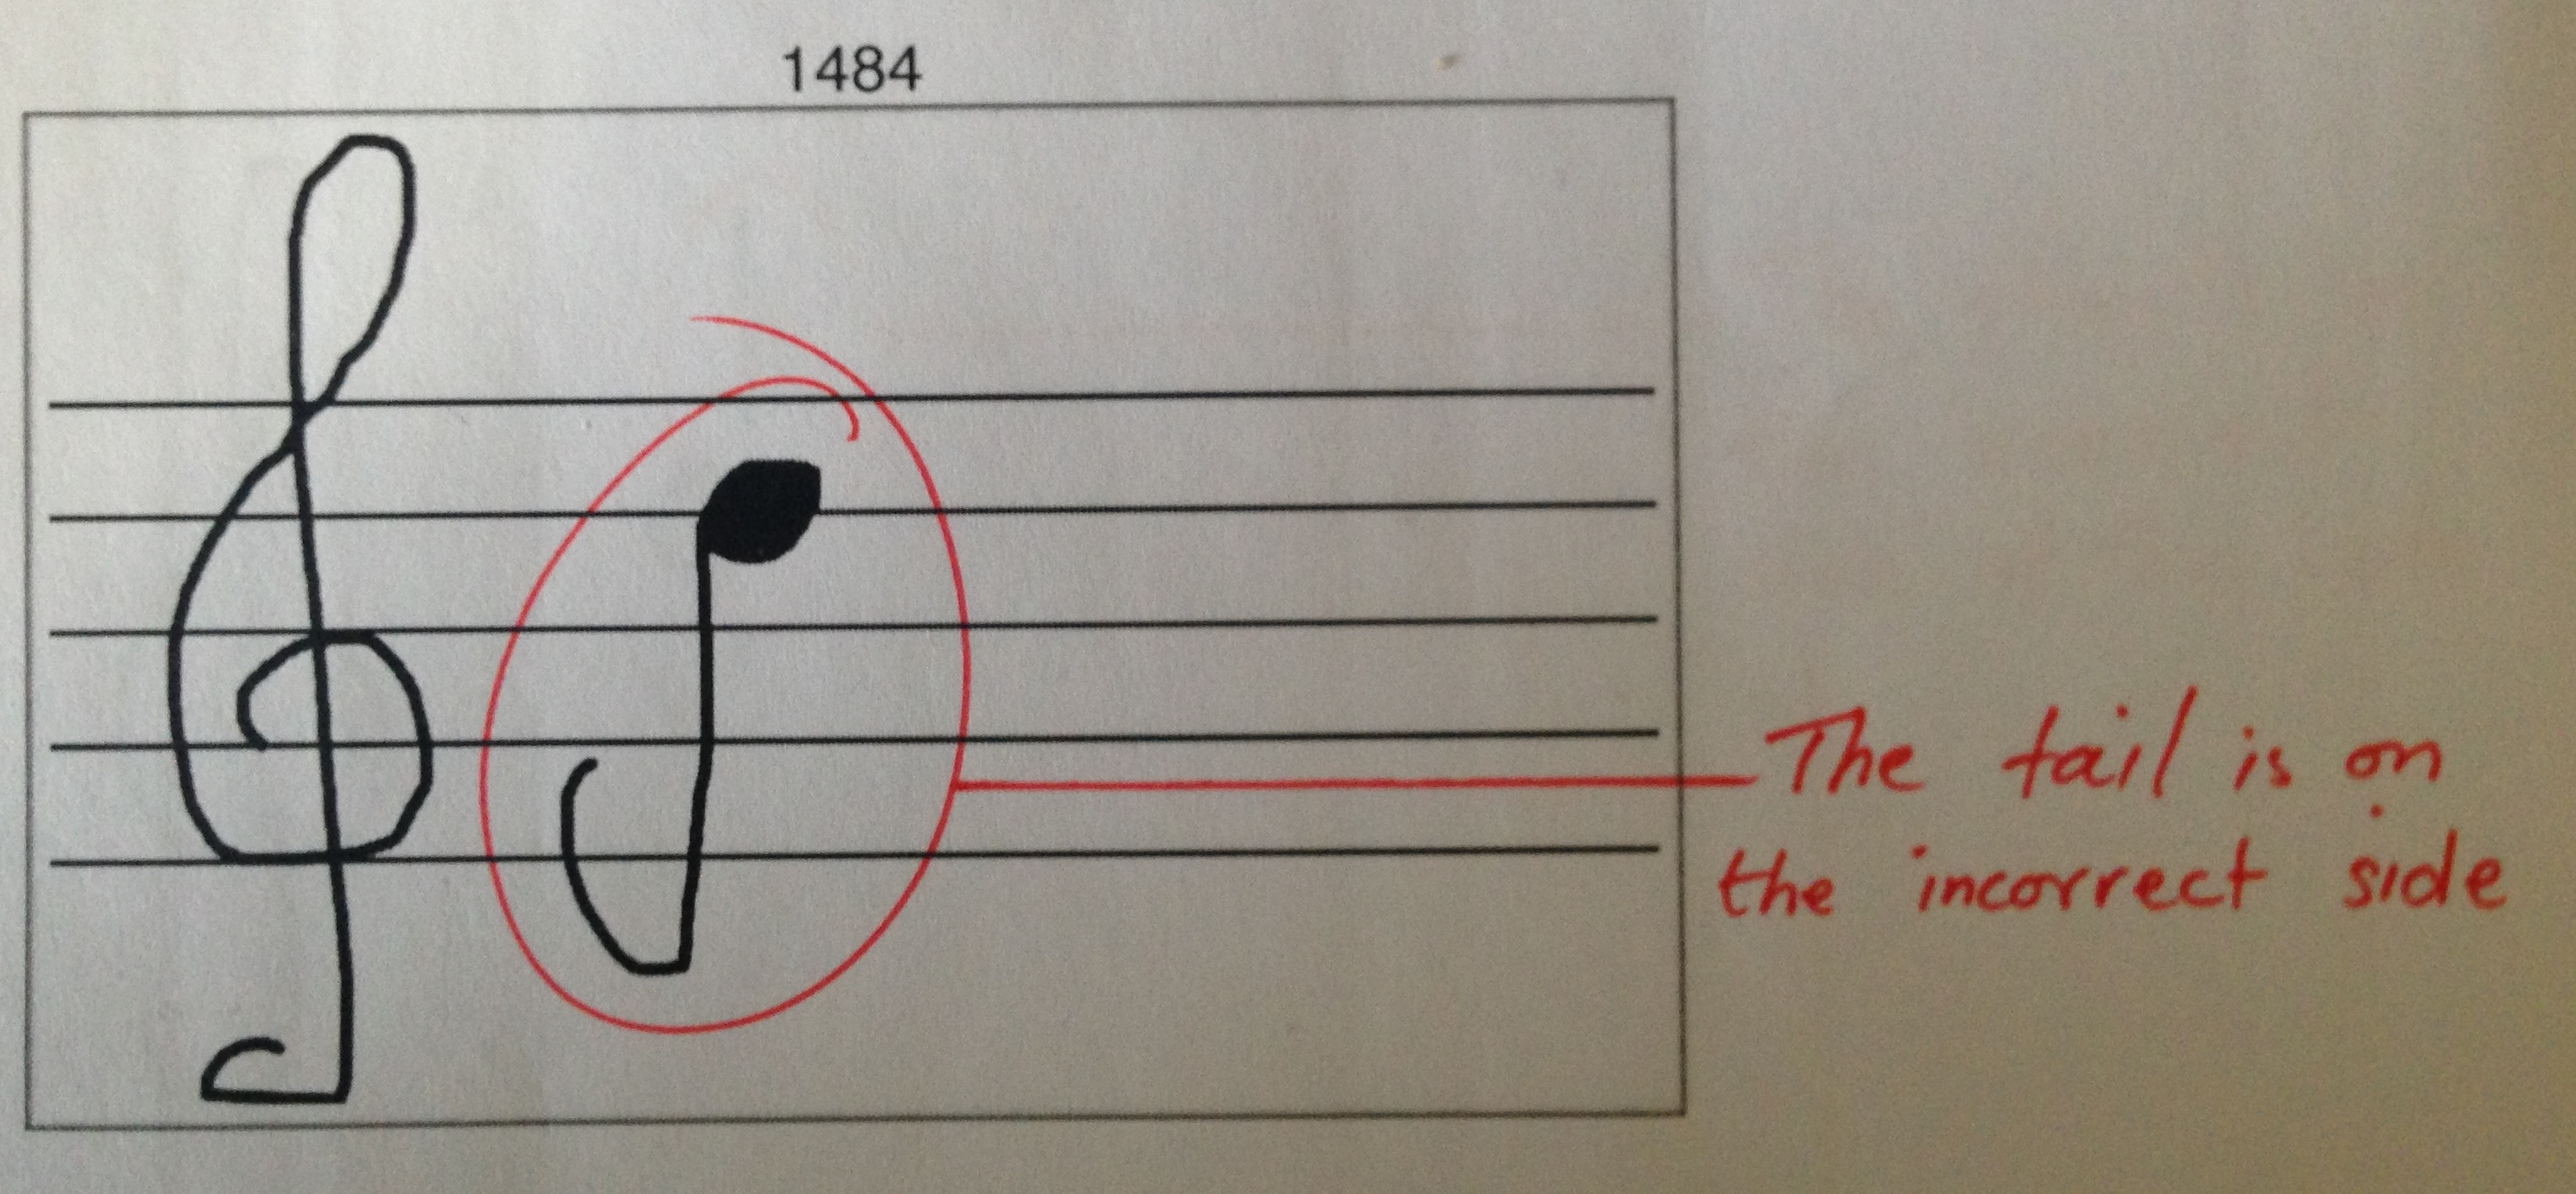
\includegraphics[width=\linewidth]{gfx/photos/teacher-bad-quavertail-side.jpg}
  \caption{Teacher's annotation of a bad quaver tail side}
  \label{fig:teacher-example-quaver-wrong-side}
\end{figure}